% \documentclass[preview]{standalone} % for final output:
\documentclass[landscape]{article}
\usepackage[margin=0.5in]{geometry} % Adjusts the margins and sets landscape mode
\usepackage{graphicx} % Required for inserting images

\usepackage{amsmath,amssymb,amsthm}
\usepackage{tikz}



% Define colors here
\definecolor{darkred}{rgb}{0.65,0,0}
\definecolor{medred}{rgb}{0.7,0,0}
\definecolor{purple}{rgb}{0.4,0,0.4}
\definecolor{lightred}{rgb}{1, 0.5, 0.5}    % Light red
\definecolor{lightblue}{rgb}{0.5, 0.5, 1}   % Light blue
\definecolor{lightpurple}{rgb}{0.75, 0.5, 0.75} % Light purple

\begin{document}



\begin{tikzpicture}

    \draw[line width = 2pt, fill = gray] (3, -8) circle (0.75);
    \node[text = white] at (3, -8) {\Large $\mathbf{x}_T$};
    \node at (3, -6.75) {\large $\mathcal{N}(0,\,\textbf{\text{I}})$};
    \begin{scope}[local bounding box=image box]
        \node at (3, -12) {
\includegraphics[width = 2cm]{xlasttv4.jpg}};
    \end{scope}
    % Now draw the border around the specific local bounding box
    \draw [white, rounded corners=0.5cm, line width=0.2cm] 
    (image box.north west) -- 
    (image box.north east) --
    (image box.south east) --
    (image box.south west) -- cycle
    ;
    

    \draw[ultra thick, ->] (4, -8) -- (4.5,-8);
    \draw[fill = black, ultra thick] (4.75, -8) circle (0.05);
    \draw[fill = black, ultra thick] (5, -8) circle (0.05);
    \draw[fill = black, ultra thick] (5.25, -8) circle (0.05);
    \draw[ultra thick, ->] (5.5, -8) -- (6,-8);

    \draw[line width = 2pt, fill = darkred] (7, -8) circle (0.75);
    \node[text = white] at (7, -8) {\Large $\mathbf{x}_{t}$};
    \begin{scope}[local bounding box=image box]
        \node at (7, -12) {
\includegraphics[width = 2cm]{xinttprimev5.jpg}};
    \end{scope}
    % Now draw the border around the specific local bounding box
    \draw [white, rounded corners=0.5cm, line width=0.2cm] 
    (image box.north west) -- 
    (image box.north east) --
    (image box.south east) --
    (image box.south west) -- cycle
    ;
    

    \draw[ultra thick, ->] (7.75,-7.25) -- (9.25,-5.75);
    \draw[line width = 2pt, fill = medred] (10, -5) circle (0.75);
    \node[text = white] at (10, -5) {\Large $\mathbf{x}_{t-1}'$};
    \node at (7.5, -6.25) {\large $p_{\theta}(\mathbf{x}_{t-1}'|\mathbf{x}_t)$};
    
    
    \begin{scope}[local bounding box=image box]
        \node at (10, -1.75) {
\includegraphics[width = 1.5cm]{xinttprimev4.jpg}};
    \end{scope}
    % Now draw the border around the specific local bounding box
    \draw [white, rounded corners=0.5cm, line width=0.2cm] 
    (image box.north west) -- 
    (image box.north east) --
    (image box.south east) --
    (image box.south west) -- cycle
    ;
    
    
    \draw[ultra thick, ->] (10.75,-5.75) -- (12.25,-7.25);
    \draw[line width = 2pt, fill = purple] (13, -8) circle (0.75);
    \node[text = white] at (13, -8) {\Large $\mathbf{x}_{t-1}$};
    \begin{scope}[local bounding box=image box]
        \node at (13, -12) {
\includegraphics[width = 2cm]{xinttprimev4.jpg}};
    \end{scope}
    % Now draw the border around the specific local bounding box
    \draw [white, rounded corners=0.5cm, line width=0.2cm] 
    (image box.north west) -- 
    (image box.north east) --
    (image box.south east) --
    (image box.south west) -- cycle
    ;
    

    \draw[ultra thick, dash pattern=on 3pt off 3pt, ->] (15.25,-5.75) -- (13.75,-7.25);
    \node at (15.5, -6.75) {\large $q(\mathbf{y}_{t-1} | \mathbf{y})$};
    \draw[line width = 2pt, fill = lightblue] (16, -5) circle (0.75);
    \node[text = white] at (16, -5) {\Large $\mathbf{y}$};
    \begin{scope}[local bounding box=image box]
        \node at (16, -1.75) {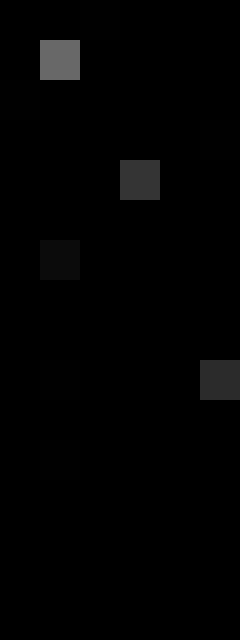
\includegraphics[width = 1.5cm]{yinttprimev5.jpg}};
    \end{scope}
    % Now draw the border around the specific local bounding box
    \draw [white, rounded corners=0.5cm, line width=0.2cm] 
    (image box.north west) -- 
    (image box.north east) --
    (image box.south east) --
    (image box.south west) -- cycle
    ;

    \draw[ultra thick, rounded corners, red, dash pattern=on 3pt off 3pt] (8.75,-4) rectangle (17.25,-9);
    \node at (13, -3.25) [align=center, text width=6cm] {\large \textbf{Latent Variable} \\ \textbf{Refinement}};


    \draw[ultra thick, ->] (19, -5) -- (17.5, -5);
    \node at (20.5, -5) {\large $\mathrm{Nd_{0.8}Sr_{0.2}NiO_{2}}$};
    

    \draw[ultra thick, ->] (14, -8) -- (15.5,-8);
    \draw[fill = black, ultra thick] (15.75, -8) circle (0.05);
    \draw[fill = black, ultra thick] (16, -8) circle (0.05);
    \draw[fill = black, ultra thick] (16.25, -8) circle (0.05);
    \draw[ultra thick, ->] (16.5, -8) -- (18,-8);
    
    \draw[line width = 2pt, fill = lightpurple] (19, -8) circle (0.75);
    \node[text = white] at (19, -8) {\Large $\mathbf{x}_0$};
    \begin{scope}[local bounding box=image box]
        \node at (19, -12) {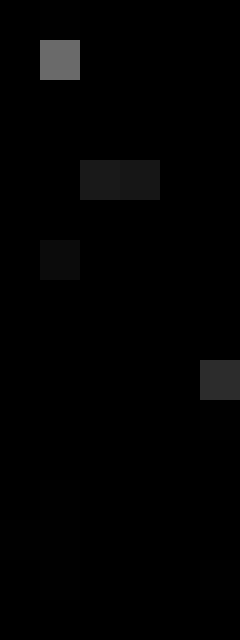
\includegraphics[width = 2cm]{xinttprime6.jpg}};
    \end{scope}
    % Now draw the border around the specific local bounding box
    \draw [white, rounded corners=0.5cm, line width=0.2cm] 
    (image box.north west) -- 
    (image box.north east) --
    (image box.south east) --
    (image box.south west) -- cycle
    ;
    \draw[ultra thick, ->] (20, -8) -- (21.5, -8);
    \node at (24.15, -8) {\large $\mathrm{O_{2.02}Co_{0.48}Ni_{0.44}Sr_{0.21}Nd_{0.84}}$};

    
    
\end{tikzpicture}


\end{document}
